\documentclass[a4paper]{report} % estilo do documento

\usepackage[utf8]{inputenc} %encoding do ficheiro
\usepackage[portuges]{babel} % para língua portuguesa
\usepackage{graphicx} % para importar imagens

\begin{document}

\title{Relatório Trabalho Prático LI1}
\author{Grupo 071\\
\\
Ricardo Silva a84123 e Rui Mendes a83712}
\date{\today}

\begin{figure}[tb]
\begin{center}

\includegraphics[width=13cm, height=10cm]{Capa.png}
\end{center}

\end{figure}

\maketitle



\tableofcontents

\listoffigures

%% Introdução
\chapter{Introdução}

  \section{Contextualização}
  O Projeto deste ano da disciplina de LI1 corresponde a uma implementação de uma variável do jogo Micro Machines™, lançado originalmente em 1991 pela Codemasters™ e distribuido entretanto por várias plataformas.
  
  Este jogo consiste em corridas simples com carros em 2d, em que o utilizador controla um deles através das setas no teclado, o jogo original porta mais caracteristicas e funcionalidades, mas a base essencial para o projeto consistia apenas nas funcionalidades mais básicas deste.
  \section{Motivação}
  Iniciamos este trabalho, não só com o objetivo de cumprir as tarefas usando as ferramentas e conhecimentos que obtive-mos nas aulas de PF, mas também como uma forma de aprender e descobrir mais num ambiente prático, possiblitando-nos assim uma forma de por-mos em prática o que aprendemos durante o semestre, bem como descobrir novas ferramentas e aplicações na linguagem usada.
  
  \section{Objectivos}
  O propósito do do projeto era o de fazer a implementação referiada da introdução em haskell, por isso, nessa mesma linguagem tivemos de resolver várias tarefas orientadas pelos professores com o fim de obter-mos um resultado funcional e de certo modo, relativo ao jogo original.
  Essas mesmas tarefas tinham também cada uma um objetivo, pode-mos portanto ter cada uma como a construção de uma ferramenta necessária ao funcionamente final do jogo. Depois de todas estas completas tinha-mos posteriormente de fazer um "encaixe", para que juntas, gerassem o jogo em si.

%% Análise de Requisitos e Especificação do Problema
\chapter{Análise de Requisitos}


\section{Fase 1}
A primeira fase corresponde principalmente ao desenvolvimento da estrutura que os carros percorrem, aqui denominados de mapas, nesta fase 
foram estes o principal tópico de trabalho, a conpreensão,definição e validação destes correspondeu á maior parte da tarefa, sendo que, já na ultima tarefa desta mesma fase, foi implementada a interação dos mesmos com os carros.

\subsection{Tarefa 1 - Construir Mapas}
Na primeira tarefa o tinhamos como objetivo definir um mapa, isto é, uma lista do tipo ((Int,Int)Orientação)[[Peca]] ((data Peca) e (data Orientação) pré definidas), através de umalista do tipo [Movimento] ((data Movimento) também pré definido), correspondendo o par de inteiros á posição inicial dos carros na corrida.

Com estas informação, e sendo-nos indicados que os mapas deveriam ser rectangulares, isto é, todas as listas de peças deviam ter o mesmo comprimento e que todas os "espaços" não preenchidas por peças da "pista" deveriam ser ocupados por peças de lava de altura 0, concluimos que seriam necessárias funções que, a partir da lista de passos nos fornecesseam as seguintes informações:

\begin{enumerate}
\item Dimensão do mapa
\item Local e orientação de partida
\item Posição e Tipo das peças do "caminho"
\end{enumerate}
As informações contidas nos items 1 e 2 eram já dadas por funcões pré definidas, cabeu-nos portanto a nós, definir um conjunto de funções para obter o ponto 3 e posteriormente concatenar toda esta informação.

\subsection{Tarefa 2 - Validar mapas}
Na segunda tarefa tinhamos o objetivo de verificar de um dado mapa era ou não válido, para isto tivemos de definir uma função que, dado um mapa, retornava um variável do tipo Bool, True se o mapa fosse válido e falso em caso contrário, para que fosse válido, o mapa deveria obedecer ás seguintes condições:
\begin{enumerate}
\item A orientação inicial é compativel com a primeira peça
\item Existe apenas um percurso e todas as peças fora do percurso são do tipo lava 
\item O percurso deve acabar na mesma peça onde começou
\item A orientação final é compativel com a orientação inicial
\item Todas as peças do percurso ligadas entre sim têm alturas compativeis
\item Todas as peças do tipo lava estão a altura 0
\item O mapa é sempre rectangular e rodeado por lava
\end{enumerate}
Com isto em mente, tivemos portanto a tarefa de definir funções que testassem todas estas condições, e por fim, uma que através destas, verificasse todas as condições em simultâneo.

\subsection{Tarefa 3 - Movimentar o carro}
A tarefa 3 tinha com objetivo a implementação da mecânica do jogo, , isto é, o movimento do carro e a sua interação com o mapa.
Para isto tinha-mos como objetivo definir uma função, que, recebendo um Carro, um Mapa e um Tempo, nos devolvia uma variável do tipo Maybe carro, devolvendo um carro com a mesma direção, mas com posição e velocidade variável dependendo das colisões ou Nothing no caso do carro ter sido destruido. 

Para a concretização deste objetivo guiamo-nos pelas seguintes regras:
\begin{enumerate}
\item Um carro colide quando: 
\begin{enumerate}
\item Atinge uma estremidade de uma peça que através dessa mesma estremidade é adjacente a uma peça com maior altura
\item Atinge a "hipotenusa" de uma curva que se encontra a altura negativa
\end{enumerate}
\item A colisão rege-se pelas seguintes regras
\begin{enumerate}
\item A velocidade varia de (x,y) para (-x,y) quando anterior colisão (a) é feita através de uma extremidade lateral da peça
\item A velocidade varia de (x,y) para (x,-y) quando anterior colisão (a) é feita através de uma extremidade vertical da peça
\item O vetor sofre uma reflexão tendo em conta o vetor normal à "hipotenusa" da curva e o vetor velocidade com que o carro colide com essa mesma "hipotenusa"
\end{enumerate}
\item Um carro é destruido quando:
\begin{enumerate}
\item Atinge uma estremidade de uma peça que através dessa mesma estremidade é adjacente a uma peça com menor altura, isto é "cai".
\item Atinge uma estremidade de uma peça de altura 0, que através dessa mesma estremidade é adjacente a uma peça lava, isto é, transita até a lava. 
\end{enumerate}

\end{enumerate}

\label{sec:analisefase1}

\section{Fase 2}
Na fase 2 definimos a última função necessária para completar a atualização do estado do carro, e definimos uma implementação do jogo em Gloss, como esta fase permitiu uma maior liberdade na implementação de funções e funcionalidades, maior parte, iremos tratar aqui apenas os requisitos básicos das funções e completar no Capitulo 3. No final tivemos também de implementar uma estratégia de corrida, que, devido também á sua natureza liberal, será melhor tratada no último capítulo.

\subsection{Tarefa 4 - Atualizar Estado}
O objetivo nesta tarefa foi de definir a função que, dado um Tempo,um Jogo (mapa,pista,carros,nitros,historico), O indice de um jogador(a sua posição na lista de carros,nitros e no histórico) e uma Ação (acelerar,travar,esquerda,direita,nitro) nos retornava o estado do Jogo decorrido o tempo indicado.
Para realizar essa atualização será então necessário definir primeiro a atualização das partes constituintes do jogo:

\begin{enumerate}
\item Atualizar o vetor velocidade, que é calculado através da soma de todas as forças que atuam no carro, calculadas por sua vez através das propriedades da pista(k-atrito,k-pneus,k-acel,k-peso,k-nitro,k-roda) sendo elas:

\begin{enumerate}
\item Força de atrito: obtida como uma percentagem da velocidade inicial (dada por
k-atrito), com sentido oposto à velocidade;
\item Força de aceleração (ou travagem): com norma dada por k-acel e com a
direção e sentido (ou oposto) do carro;
\item Força da gravidade (usada apenas em rampas): de acordo com a constante
k-peso, na direção do declive;
\item Força dos pneus: vetor perpendicular à direção do carro, no sentido oposto à
velocidade, com norma dada por seno(angulo da direcao à velocidade inicial) x k-pneus ; 
\end{enumerate}

\item Atualizar a direção do carro no carro de "esquerda" ou "direita" serem verdadeiros de acordo com o k-roda
\item Atualizar a quantidade de nitro(Maybe Int) caso este não seja "Nothing", isto é, está aplicado a algum dos jogares (ao próprio ou não)
\end{enumerate}

Para isto ouve a necessidade de efetuar várias funções para efetuar os calculos e a função final que, através delas realizasse a atualização do Jogo.

Esta Tarefa, juntamente com a 3, permitir-nos-á efetuar a movimentação do carro na pista, através de sucessivas atualizações da posição, direção e velocidade do carro na que serão concatenadas na próxima.

\subsection{Tarefa 5 - Implementação do jogo em Gloss}
Esta tarefa tinha um objetivo essencial, fazer a implementação do jogo com base na biblioteca Gloss, para isso, houve a necessidade de comprir 3 sub-objetivos, desenvolver uma função que nos fornecesse os dados do jogo funcional (com base nas tarefas 3 e 4), uma outra que através desses mesmos dados desenvolvesse uma "projeção" gráfica representativa do jogo e finalmente, uma série de funções que permitissem ao jogador interagir com o jogo (através de comandos no teclado).

Por fim, devido ao funcionamento da implementação em Gloss, tivemos de contruir um conjunto de funções com vista a atualizar o "Estado" do jogo, isto é, a mudança que este sofria entre cada mudança de tempo indicada na função principal definida na Tarefa 5.

Além do objetivo inicial, a Tarefa 5 era sobretudo uma tarefa livre, deixando muito á nossa criatividade, por isto mesmo também, os problemas e os objetivos desta parte da tarefa estão colocados durante o desenvolvimento da nossa solução.

\subsection{Tarefa 6 - Implementação de uma estratégia de corrida}
Na tarefa 6 tinha-mos como objetivo implementar um bot capaz de percorrer o caminho no menor tempo possivel, isto é, uma série de funções que, recebendo um jogo, um tempo de ação e o indice do jogador, determinassem a ação correta a desempenhar por esse jogador, com isto em mente, esta é a tarefa mais baseada em testes, pois só assim é possivel corrigir as funções, portanto, muitos dos problemas descobertos estão também contidos durante a implementação da nossa solução.

%% Descrição da Solução Desenvolvida
\chapter{A Nossa Solução}
\label{sec:solucao}
\subsection{Tarefa1}
Nesta tarefa, devido á necessidade de construir um "caminho" através de uma lista de passos, dividimos o problema em duas partes principais, "Qual a peça seguinte?" e "Onde colocar a peça seguinte", para isso desenvolvemos série de funções que dependendo do problemas colocado, nos davam informações sobre a nova peça dependendo do "passo" dado, isto é, a nova orientação, a posição da peça seguinte, o tipo da peça seguinte, a altura da peça seguinte, todas estas culminaram na função "caminhoToBlocos" que é do tipo
\begin{verbatim}
caminhoToBlocos :: Bloco -> Caminho -> [Bloco]
\end{verbatim}
Isto é recebe um bloco (o incial, dado por uma outra função,"prim-peca") e produz a lista de blocos correspondentes ao caminho.

Depois disto, houve a necessidade de colocar estes blocos no tabuleiro, para isso foi definada a função "BlocosToTabuleiro" do tipo
\begin{verbatim}
blocosToTabuleiro :: [Blocos] -> Tabuleiro -> Tabuleiro
\end{verbatim}
Que portanto, traduz estes blocos para um tabuleiro (Sendo este um tabuleiro contendo apenas só lava, criado também por uma outra função, "tabuleiroInit", esta constroi um tabuleiro com lava de acordo com a dimensão do mapa, dimensaão esta dada por uma função pré fornecida).

Tudo isto culminou na função constrói:
\begin{verbatim}
constroi::Caminho->Mapa
constroi [] = Mapa ((partida []), Este) (tabuleiroInit(dimensao []))
constroi (p:c) = Mapa ((partida (p:c)), Este) (blocosToTabuleiro (caminhoToBlocos...
                       ...(prim_peca (p:c)) c) (tabuleiroInit(dimensao (p:c))))
\end{verbatim}
(A função partida é também pré fornecida)

\newpage

\subsection{Tarefa2}
Na tarefa 2 tinhamos como objetivo, verificar a validade de um mapa através das condições pré definidas.As condição 1,7 e parte da 6 poderam ser conferidas através de funções singulares,"oriInitpossivel" "check-rectangulo" e "bordersLava". 
\begin{verbatim}
oriInitpossivel::Orientacao->Peca->Bool
check_rectangulo:: Tabuleiro->Bool
bordersLava::Tabuleiro->[Int]->Bool
\end{verbatim}
Porém as restantes condições sentiam todas a mesma necessidade, tinhamos de descobrir o caminho através do tabuleiro, para isso definimos um conjunto de funções que, seguindo a posição e orientação de uma peça, determinassem a orientação("proxOri"),posição ("move"(definida na Tarefa anterior)) e validade de tipo e altura, atráves destas podia-mos como que "seguir" o caminho, e assim, verificar todas as condições em falta, logo no primeiro "passo" podemos verifcar a condição 1, após definir-mos uma função que "guarda" todas as posição e peças orientadas pelas funções anteriores:
\begin{verbatim}
guardaPosVal::Mapa->(Peca,Posicao)->Orientacao->[Posicao]
\end{verbatim}
Pode-mos usar esta mesma lista para verificar as seguintes condições, ao "chamar" a função, na definição da lista   podemos verificar a compatibilidade das alturas e peças(condição 5),através do primeiro e último elemento dessa lista podemos verificar as condições 3 e 4, e posteriormente verificando todas as peças que não fazem parte do percurso concluimos a condição 6 ao mesmo tempo que completamos a 2.

A função final ficou do género:
\begin{verbatim}
valida :: Mapa -> Bool
valida m@(Mapa (posi,oi) t) = oriInitpossivel oi (getPeca t posi)&&
                              check_rectangulo t&&
                              bordersLava t [0..(ty-1)]&&
                              verificaTudoLava t (allPos (tx,ty)) posValidas
                              && head posValidas == last posValidas
                              where (tx,ty) = dimensaoTabuleiro t
                                    posValidas = (guardaPosVal ... 
                                               ...m((getPeca t posi),posi)oi)
\end{verbatim}
\subsection{Tarefa3}
Nesta tarefa tinha-mos o objetivo de determinar a posição e velocidade de um carro passado um determinado tempo, para isso tinhamos de definir a função: 
\begin{verbatim}
movimenta::Tabuleiro->Tempo->Carro->Maybe Carro
\end{verbatim}
Que devolva o estado do carro passado um determinado tempo ou Nothing caso este seja destruido durante esse tempo.

Começamos por definir a função foraPeca:
\begin{verbatim}
foraPeca::Tabuleiro->Ponto->Velocidade->Tempo->Bool
\end{verbatim}
Dada a posição do carro, a sua velocidade e um tempo, determina se o carro atinge uma das extremidades da peça antes do tempo acabar.


Posteriormente definimos um conjunto de funções de maneira a determinar esse mesmo ponto sendo estas:
\begin{verbatim}
obterDirVel::Velocidade->(Orientacao,Orientacao)
obterMenorTempoR::Orientacao->Ponto->Velocidade->(Double,Orientacao)
menorTempo::(Double,Orientacao)->(Double,Orientacao)->(Double,Orientacao)
\end{verbatim}
Que culminam na seguinte:
\begin{verbatim}
pontoSaidaGeral::Ponto->Velocidade->(Ponto,Tempo,Orientacao)
pontoSaidaGeral p v = ((step p v novoT),novoT,ladoBateu)
                               where (a,b) = obterDirVel v
                                     novoT = fst(menorTempo (obterMenorTempoR...
                                     ...a p v)(obterMenorTempoR b p v))
                                     ladoBateu = snd(menorTempo (obterMenorTempoR... 
                                     ...a p v) (obterMenorTempoR b p v))
\end{verbatim}
Assim, a fução "obterDirVel" dá-nos as duas orientações de uma velocidade,isto é por exemplo: (Sul,este) no caso das duas coordenadas serem positivas, sabendo isto, o ponto de saida do vetor velocidade da peça fica resumido a duas retas, neste caso, a extremidade direita ou a de baixo, a função "obterMenorTempoR" calcula esses dois pontos, e a função "menorTempo", seleciona o menor desses dois, sabemos que esse ponto faz parte da peça, porque no caso do impacto ser feito fora da peça, isto é por exemplo, intercetar a reta definida pela extremidade direita a uma altura inferior ás validas na peça, essa interseção só seria possivel após intercetar a reta inferior, numa abcissa compativel com a peça, ponto esse, que será o dado pela terceira função.

A partir deste ponto, temos de determinar o que acontece ao carro,para isso definimos a função "decideMudança"
\begin{verbatim}
decideMudanca::Peca->Orientacao->Peca->Mudanca
\end{verbatim}
Sendo que:
\begin{verbatim}
data Mudanca = Horizontal | Vertical | Diagonal | Segue | Morre deriving (Show,Eq)
\end{verbatim}
Esta função testa toda a larga escala de casos possiveis e devolve um dos 6 tipos de mudança possiveis que deverá ser efetuado a partir daquele ponto, assim, definimos posteriormente a função "mudaVelocidade"
\begin{verbatim}
mudaVelocidade::Tipo->Velocidade->Mudanca->Velocidade
\end{verbatim}
Esta função, dependedo do tipo da peça (Importante para as curvas no caso duma colisão diagonal), irá aplicar a devida alterção ao vetor velocidade.Tendo então todas as peças definidas, o encaixe da função "movimenta", foi feito da seguinte maneira:
\newpage
\begin{verbatim}
movimenta :: Tabuleiro -> Tempo -> Carro -> Maybe Carro
movimenta m t (Carro {posicao=p@(px,py),direcao=d,velocidade=v}) |...
                                                                 |...
                                                                 |...


...| foraPeca m p v t && tipoMudanca == Morre = Nothing
...| foraPeca m p v t = movimenta m (t-b) colidiu
...| otherwise = Just e
   where (a,b,c) = pontoSaidaPeca m p v
                  (_,_,ori) = pontoSaidaGeral p v
                  tipoMudanca = decideMudanca (whichPeca p m) ori (getPeca m... 
                  ...(move (floor px,floor py) ori))
                  colidiu = (Carro {posicao=step a novaV (0.000000000001),direcao=d,...
                  ...velocidade=novaV})             
                  e = (Carro {posicao=(step p v t),direcao=d,velocidade=v})
                  novaV = (mudaVelocidade (getTipo(whichPeca p m)) v tipoMudanca)
\end{verbatim}
\subsection{Tarefa4}
O trabalho desenvolvido neste função, fez-se sobretudo sobre vetores, por, isto e devido á existência de forças com angulos variáveis á velocidade começamos por definir funções auxiliares para o calculo 
sendo elas:
\begin{verbatim}
toRadian::Double->Double
cartToPolar::(Double,Double)->(Double,Double)
polarToCart::(Double,Double)->(Double,Double)
\end{verbatim}
Que nos permitirão fazer os cálculos de acordo com o enunciado.Consequentemente, definimos essas mesmas funções de cálculo, sendo:
\begin{verbatim}
vAcel::Carro->Acao->Double->Tempo->Velocidade
vAtri::Carro->Double->Tempo->Velocidade
vPneu::Carro->Double->Tempo->Velocidade
vPeso::Tabuleiro->Carro->Double->Tempo->Velocidade
\end{verbatim}
Dando-nos cada uma o vetor que será necessário somar á velocidade do carro de modo a obter o resultado da aplicação dessa mesma força,e semelhante a essas mas com especificações diferentes, a função "ativaNitro":
\begin{verbatim}
ativaNitro::Int->[Carro]->Double->Tempo->[Velocidade]
\end{verbatim}
Que, recebendo o indice do carros que sofre o Nitro, a lista dos carros, a força do Nitro e o tempo durante o qual este é aplicado, nos devolve uma lista com os vetores resultantes das forças de Nitro, cujos teremos de somar á velocidade(Apenas um desses vetores será diferente de 0 pois estamos apenas a lidar com o Nitro aplicado a 1 jogador)

Consequente a esta a função "atualizaNitro"
\begin{verbatim}
atualizaNitro::Int->Tempo->[Tempo]->[Tempo]
\end{verbatim}
Esta recebe o indice do jogador que usa o nitro, o tempo durante o qual o faz, a lista dos tempos restantes de nitro, e devolve a lista retirando o respetivo tempo de Nitro ao jogador que o usou.

De modo a atualizar a velocidade dos carros houve a necessidade de definir a função "novaV"
\begin{verbatim}
novaV::Tabuleiro->Acao->Carro->Propriedades->Tempo->Velocidade
\end{verbatim}
Que faz o cálculo de todas as forças constantes e as adiciona á velocidade do carro

Tal como a função "adicionaV"
\begin{verbatim}
adicionaV::Carro->Velocidade->Carro
\end{verbatim}
Que adiciona um certo vetor(Neste caso a resultante da força do Nitro) á velocidade de um carro.

Com isto definimos a função "atualizaV"
\begin{verbatim}
atualizaV::Tempo->Jogo->Int->Acao->Jogo
\end{verbatim}
Que aplica a função novaV ao jogador indicado, e, no caso de o jogador fazer uso do Nitro, aplica também a funçao adicionaV com a sua resultante(dada pela função ativaNitro) ao jogador destino.

Velocidade tratadas, restava apenas implementar uma solução para atualizar as direções, para isto começamos pela função "adicionaD",
\begin{verbatim}
adicionaD::Acao->Double->Tempo->Carro->Carro
\end{verbatim}
Que altera a direção de um carro dada uma ação, a constante kRoda, um tempo e o carro que se pretende "rodar".Esta é usada na função atualizaD que, recebe semelhante á anterior recebe um tempo e uma ação, mas ao invés da constante k-roda e um carro, recebe um jogo e o indice de um jogador, assim, aplica a função "adicionaD" ao jogador constante no indice e devolve o jogo feita essa alteração.
\begin{verbatim}
atualizaD::Tempo->Jogo->Int->Acao->Jogo
\end{verbatim}
Por fim houve apenas a necessidade de definir a função "guardaPos" que guarda as posições porque um carro passa,não é usada nesta tarefa, mas será útil durante o desenvolvimento da tarefa 5 e 6 por estar presente na função "atualiza".
\begin{verbatim}
guardaPos::Carro->[Posicao]->[Posicao]
\end{verbatim}

Por fim definimos a função "atualiza"
\begin{verbatim}
atualiza :: Tempo -- ^ a duração da ação
         -> Jogo  -- ^ o estado do jogo
         -> Int   -- ^ o identificador do jogador
         -> Acao  -- ^ a ação tomada pelo jogador
         -> Jogo  -- ^ o estado atualizado do jogo
atualiza t j i a = atualizaD t (atualizaV t j i a) i a
\end{verbatim}
Que concateca tudo o efetuado pelas funções anteriores.
\subsection{Tarefa5}
\subsubsection{Implementação em gloss}
O objetivo fundamental e a base da tarefa 5 era o de fazer uma implementação do jogo em Gloss, para isto eram necessárias várias peças fundamentais,definir a janela, uma função capaz de mostrar graficamente o estado do jogo, definir um estado inicial, um conjunto de funções que permitissem ao jogador interagir com o jogo e, por fim, definir uma função que atualize o estado do jogo.

Achamos adequado implementar uma janela de Dimensões 1000x1000, isto foi feito através da função:
\begin{verbatim}
wnd::Display
wnd = InWindow  "Micro Machines - World Cup Edition"
                (1000,1000)
                (500,500)
\end{verbatim}
Que também define o posicionamento incial da janela.

De seguida fizemos a definição do estado, mas este, devido á sua presença e importância durante todo o desenvolvimento da tarefa sofreu constante alterações, acabando por fim, de ficar com as seguintes caracteristicas:
\begin{verbatim}
type Estado = (Jogo,[[Picture]],[(Bool,Bool,Bool,Bool,Maybe Int)],...
[Int],[Int],Float,[Double],[Mapa],[Bool],[[Int]],Mapa,[Int],[String])
type Estado = (Jogo,[[Picture]],[(Bool,Bool,Bool,Bool,Maybe Int)],[Int]...
...,[Int],Float,[Double],[Mapa],[Bool],[[Int]],Mapa,[Int],[String]...
...,Propriedades,[Propriedades])
\end{verbatim}

O estado do Jogo(Em geral) é constitúido por um jogo, que é a proxima corrida a correr,uma lista de imagens, que que correnponde a todos os aspetos gráficos do jogo,um conjunto de Bools que definem a ação do jogador (incluindo Nitros), uma lista de Int's que possui todas as variavéis inteiras do jogo,uma lista com o número de voltas dadas por cada jogador, uma lista com os indices dos carros aleatórios a correr, um float que regista o tempo que passou, e uma lista de Double's que conta o tempo que passou desde a ultima morte de um dado jogador, uma lista de Mapas que são usados no modo campanha, uma Lista de Bool's que nos dá várias informações sobre o jogo, uma lista de listas de inteiros para identificar os jogadores em cada eliminátoria,um Mapa destinado ao modo de corrida rápida, uma lista de posições no final de cada corrida e, finalmente, um conjunto de propriedades e uma lista de conjuntos de propriedades, estes servirão para, respetivamente, alterar os temas no modo corrida rápida, e no modo campanha.

É de salientar que a atribuição aleatória, tanto de mapas como de temas é feita ao criar o Estado, isto é, ao ligar o jogo, devendo o utilizador, caso queira mudar os mapas, reiniciar o jogo.

O estado inicial é definido por:
\begin{verbatim}
estadoInicial::Jogo->[[Picture]]->Int->[Int]->Int->[Mapa]->Mapa->Estado
estadoInicial jog [flor,gelo,praia,carros,inter,bande,num,letras] nj lC tema...
...lMapas mapaR = (jog,[flor,gelo,praia,carros,inter,bande,num,letras],
                  replicate nj (False,False,False,False,Nothing),[0,0,nj,tema,0,0],
                  replicate nj 0,0,replicate nj 2,lMapas,[False,False,False],[lC],
                  mapaR,[0..(nj-1)],listaNomes)
\end{verbatim}
Que define o estado inicial tendo em conta um jogo inicial, a lista com os constituintes gráficos e o número de jogadores base.

A nivel gráfico definimos uma série de funções que permitissem ao jogador receber toda a informação que lhe fosse pertinente durante o jogo mas sem impedir causar confusão ou qualquer impedimento durante o jogo, para isso definimos as seguintes funções:
\begin{verbatim}
pecaToPic::Estado->Float->Peca->Picture
tabToPic::Tabuleiro->Tabuleiro->Estado->(Float,Float)->[Picture]
drawCars::Tabuleiro->Int->[Carro]->Estado->[Picture]
drawTempo::String->[Picture]->Tabuleiro->[Picture]
drawNitros::[Double]->[Int]->Tabuleiro->[Picture]
drawPos::Int->[Int]->Tabuleiro->[Picture]->[Int]->[Picture]
desenhaNitros::[Double]->[Maybe Int]->Estado->[Picture]
\end{verbatim}

Todas estas funções têm a função de fazer a impressão gráfica de algum elemento do jogo, sendo que, algumas das funções como dimensaoTab,scaleFactor e tempoString são são auliadas por funções que recolhem informação do jogo como:
\begin{verbatim}
dimensaoTab::Tabuleiro->(Float,Float)
scaleFactor::Tabuleiro->Float
tempoString::Float->String
\end{verbatim}
Estas funções são concatenadas na função "desenhaCorrida"
\begin{verbatim}
desenhaCorrida::Estado->Picture
\end{verbatim}
Que se serve de todas as outras e faz a impressão "completa" do jogo a quando de uma corrida em curso. 
Sendo que a função "draw" responsável pela totalidade das impressões absorve já um maior nivel de complexidade devido á implementação de funções não fundamentais á tarefa(Como por exemplo, a necessidade de mostrar o Menu ao inicar o jogo e de permitir alternar entre os modos de jogo e o Menu) que serão referidas posteriormente.


A nivel da atualização do jogo começamos por definir a função "movimentaCarros" que com base na função "movimenta" definida na tarefa3, atualiza a posição de uma certa lista de carros tendo em conta o tabuleiro,o tempo e a lista de carros, sendo que, se o carro "morrer", é colocado no centro da peça onde presentemente está, sendo que, o mesmo é também efetuado se o carro "cortar" demasiadas peças, condição que é verificada pela função "cortouCaminho":

\begin{verbatim}
movimentaCarros::Tabuleiro->Tempo->[Carro]->[[Posicao]]...
...->[Posicao]->Int->[(Carro,Bool,Bool)]

cortouCaminho::[Posicao]->[Posicao]->Bool
\end{verbatim}
Esta função, juntamente com funções como:
\begin{verbatim}
atualizaBots::Int->Jogo->Tempo->Estado->(Jogo,[Acao])
--Atualiza todos os bots existentes no jogo, devolvendo assim o jogo atualizado 
(Utilizada sempre que o jogador corre sempre contra bots, "correndo" portanto, 
tanto no modo campanha como no modo corrida rápida)

mudaHisto::[[Posicao]]->[Bool]->Int->[[Posicao]]
--Que atualiza os históricos dos Carros

deuVolta::[[Posicao]]->[[Posicao]]->[Posicao]->[Int]->([[Posicao]],[Int])
fimDoJogo::[Int]->Estado->(Estado,Bool) 
--Usadas para o funcionamento geral da corrida

proxEliminatoria::(Int,Int)->[Int]->[Int]
--Utilizada no modo campanha

trataMorto::Int->[Bool]->Estado->Estado
--Que verifica de um carro está "morto"(isto é, se sofreu a mudança para... 
...o centro da peça por morrer no próximo frame) e o coloca no estado morto...
...(isto é, inicia o temporizador que impede a ação)

trataAcaoMorto::Int->Estado->Acao->Acao
--Impede um carro que morreu recemtemente de tomar qualquer ação
\end{verbatim}

Irá servir a função "tU":
\begin{verbatim}
tU::Float->Estado->Estado
\end{verbatim}
Esta função é a responsável pela atualização automática do jogo, tendo em conta o estado atual do jogo e o tempo que se passou desde a ultima atualização, faz também uso da função atualiza definida na tarefa anterior, pois completa o funcionamento "mecânico" do jogo, a atualização geral da corrida, A velocidade dos carros, a sua direção,posição e Nitros, mas devido ás especificidades e funcionalidades da nossa implementação em particular, tal como a função draw, verifica condições e tem assim, um comportamento diferente dependendo da condição verificada.


A nivel de IO, interação com o utilizador implementamos a função iU, que recolhe todos os inputs do utilizador:

\begin{verbatim}
iU::Event->Estado->Estado
\end{verbatim}
Nesta houve a necessidades de implementar condições em cada tecla, devido também á implementação de funções extraordinárias neste caso particular o Menu, é dado como exemplo a tecla "Up":
\begin{verbatim}
KeyUp -> case getMenu e of
       2 -> if ks == Down
            then mudaAct (getAct e) True 0 e
             else mudaAct (getAct e) False 0 e
       0 -> if ks==Down then if getOption e>0
       then  mudaOption (-1) e
       else  mudaOption 0 e
       else e
       _ -> e
\end{verbatim}
Que devolve um resultado diferente no caso do utilizador estar no Menu ou não.

Tudo isto culmina na função "main"
\begin{verbatim}
main::IO()
main = do 
       mapaA <- randomMapa 
       carros <- carregaCarros
       floresta <- carregaFloresta
       gelO <- carregaGelo
       praia <- carregaPraia
       inter <- carregaMenu
       bandeiras <- carregaBandeiras
       lCarros <- baralhaCarros [0..31]
       num <- carregaNum
       letras <- carregaLetras
       lMapas <- listaMapas
       play wnd (greyN 0.4) 80 (estadoInicial (createJogo 4 (mapaA)... 
       
       ...gelo) [floresta,gelO,praia,carros,inter,bandeiras,num,letras]... 
       ...4 lCarros 0 lMapas (mapas16!!0)) draw iU tU
\end{verbatim}
Que é a responsável pela animação de todo o jogo, faz uso das funções "carrega", que são usadas para dar "load" de todas as imagens e de funções como "baralhaCarros","listaMapas" e "randomMapa" (utilizadas para o modo campanha e corrida rápida) bem como todas as funções anteriormente referidas, para assim, finalizar a implementação do jogo funcional

Referidas anteriormente durante a implementação das funções, as funçionalidades extraordinárias que implementamos no nosso jogo foram as seguintes: 
\subsubsection{Menu}
Devido á vertente criativa e á multiplicidade de funções possibilitadas nesta tarefa, decidimos criar um Menu que possibilitasse um simples acesso a todas essas, neste Menu o utilizador pode escolher a funcionalidade do jogo a lançar através de comandos nas "setas" no teclado e proceder ao seu lançamento com a tecla Enter. 
\newpage
\begin{figure}[tb]
\begin{center}
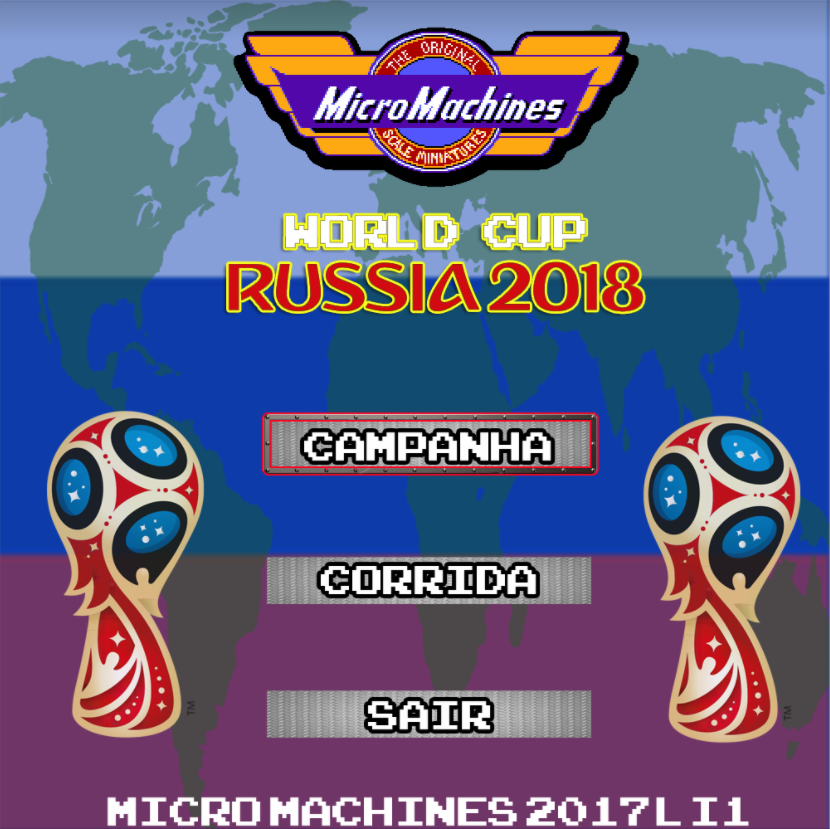
\includegraphics[width=14 cm]{Menu.png}
\end{center}
\caption{Menu}
\end{figure}
\clearpage
\subsubsection{Modo Campanha}
O modo campanha é o modo principal do jogo, neste o jogador participa num torneio contra corredores de vários paises, tem como objetivo ganhar corrida após corrida de modo a poder prossseguir no torneio, á medida que avança os corredores adversários vão aumentando em grau de dificuldade e os mapas tornam-se gradualmente mais complexos, o objetivo final do utilizador é vencer todas as corridas e tornar-se assim o campeão do mundo em Micro Machines.

Para isto começa por selecionar o pais pelo qual quer competir(Representado pela pinture do carro),
posteriormente pode verificar as partidas que serão efetuadas durante as eleminatórias, no caso de vencer a corrida, terá ao ser dispor o resultado dessa mesma eliminatória, onde poderá ver os corredores eliminados e os contra quais terá de competir, os mesmo se repete, até que, se vencer a final, irá ver o seu nome no topo da lista será congratulado.

\begin{figure}[tb]
\begin{center}
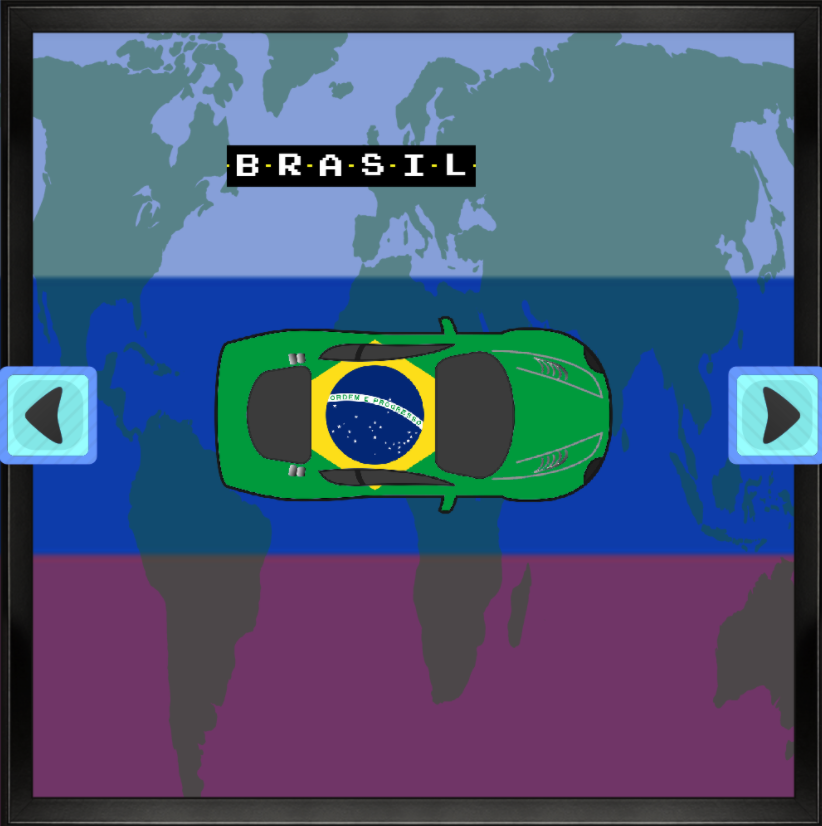
\includegraphics[width=9cm]{Sele__o.PNG}
\end{center}
\caption{Seleção de corredor}
\begin{center}
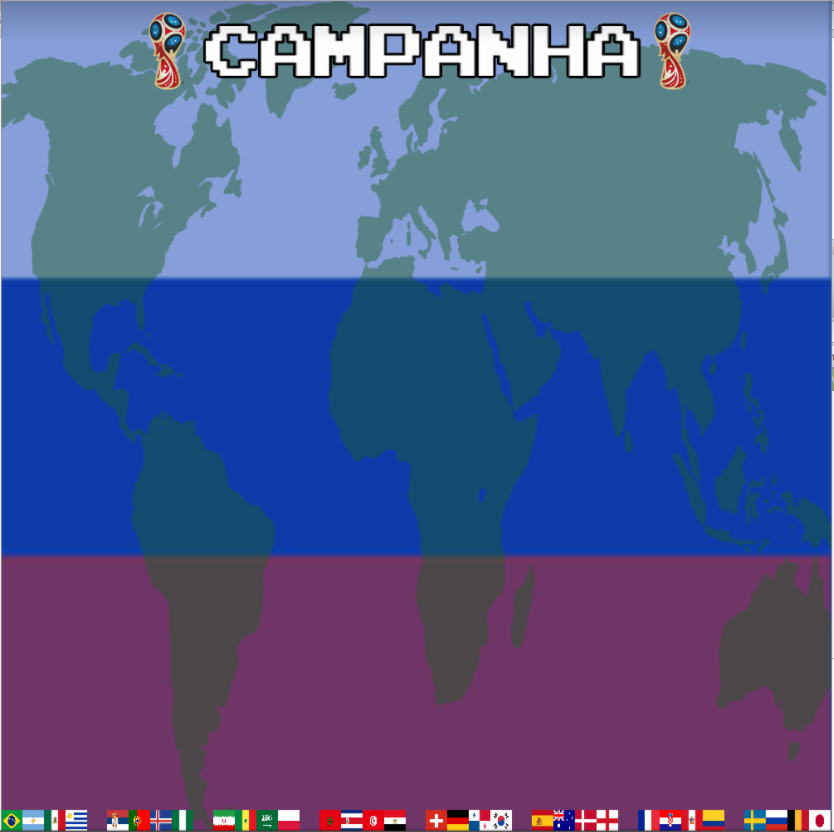
\includegraphics[width=9cm]{Inicio_Campanha.PNG}
\end{center}
\caption{Show-off da eliminatória}
\end{figure}

\vfill
\clearpage

\subsubsection{Temas}
De modo a aumentar a variabilidade do ambiente de modo a manter o jogo "fresco", resolvemos implementar uma série de temas que vão variando ao longo do modo campanha, este são "floresta","gelo", "praia" e vão sendo alternados durante o próprio modo de campanha, e têm diferentes propriedades, criando assim um novo nivel de profundidade do modo arena.

\begin{figure}[tb]
\begin{center}
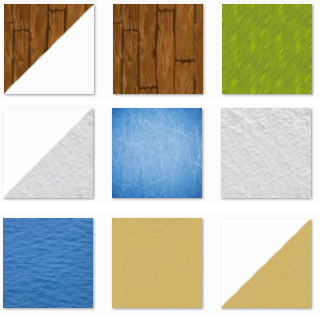
\includegraphics[width=6cm]{Temas.png}
\end{center}
\caption{Os vários temas disponiveis}
\end{figure}

\subsubsection{Modo Corrida rápida}
O modo corrida rápida é o modo mais simples e "casual" do jogo, neste o jogador percorre apenas um mapa e não tem qualquer outro propósito na corrida senão chegar em primeiro lugar, possibilitando assim, ao contrário do modo campanha um jogo mais relaxado e sem grandes objetivos e sem nada a perder.

\begin{figure}[tb]
\begin{center}
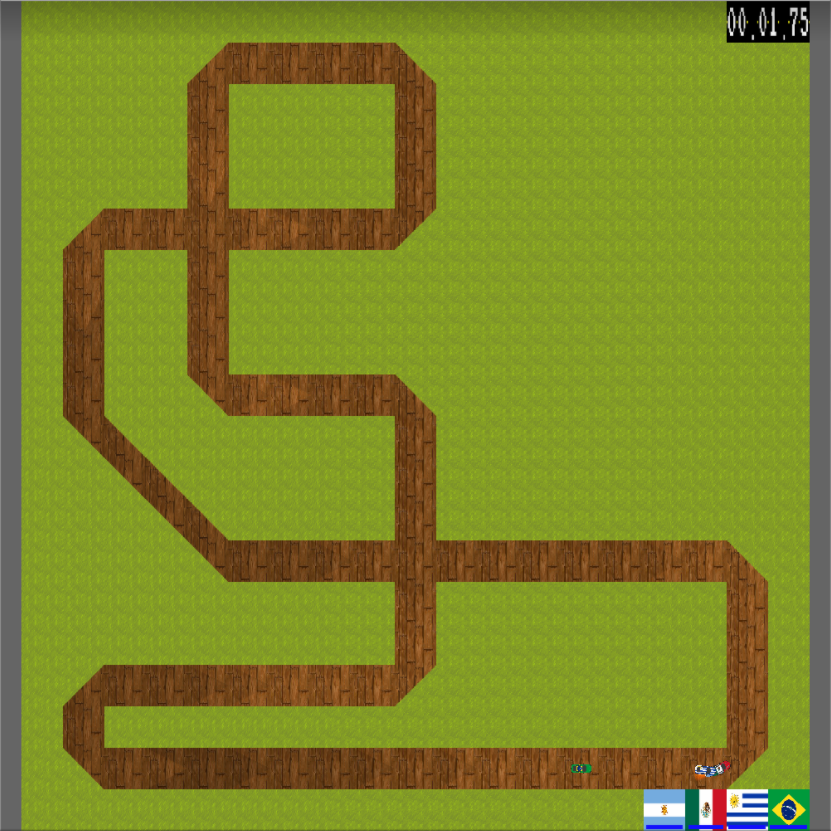
\includegraphics[width=7cm]{Corrida_r_pida.PNG}
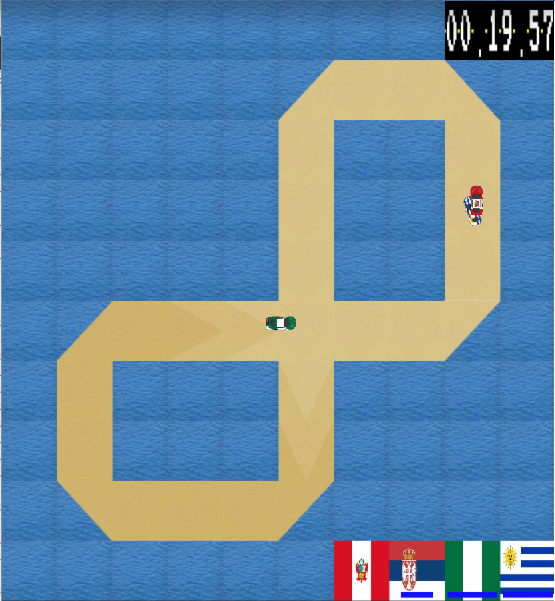
\includegraphics[width=6cm]{Praia.PNG}
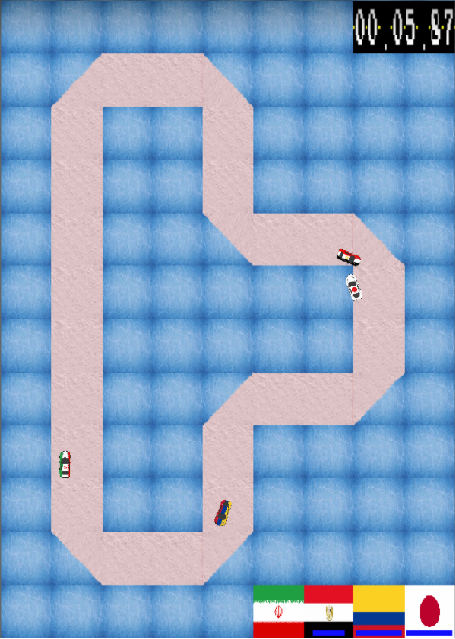
\includegraphics[width=6cm,]{Gelo.PNG}
\end{center}
\caption{Exemplo de uma corridas, em temas, respetivamente:Floresta, Praia,Gelo}
\end{figure}

\vfill
\clearpage

\subsection{Tarefa6}
O objetivo principal desta tarefa era desenvolver um bot capaz de percorrer mapas válidos, o funcionamento do bot, baseia-se em ações, por isso, antes de tudo, definimos as funções para executar essas mesmas ações:
\begin{verbatim}
viraDir::Acao
virEsq::Acao
\end{verbatim}
Definimos também as seguintes funções para auxiliar no tratamento de angulos
\begin{verbatim}
above::Double->Double->Bool
whichQuad::Double->Int
\end{verbatim}
Posteriormente definimos a função "listaAng"
\begin{verbatim}
listaAng::Tabuleiro->Posicao->Orientacao->[Posicao]->...

...(Orientacao->Peca->Peca->Angulo)->[Angulo]
\end{verbatim}
Que devolve a lista de angulos que a direção do bot deve ter tendo em conta o tabuleiro, a posição inicial, a orientação inicial e a lista de posições percorridas para o percurso.Tanto esta como as funções:
\begin{verbatim}
posAng::Propriedades->Orientacao->Peca->Peca->Angulo
aproxima::Double->Double->Acao
\end{verbatim}

Sendo que a função posAng nos devolve a melhor direção que o carro deve ter numa dada
peça, para isso recebe a orientação de entrada na peça, a peça em que está e a peça
para que se dirige, e a Função aproxima nos fornece a ação a tomar para aproximar um dado
angulo ao valor que se pretende para que posteriormente se efectue os movimentos correspondentes.

Definimos também, a nivel de angulos as funções:
\begin{verbatim}
centrado::Espaco->Ponto->Posicao->Orientacao->Bool
centra::Angulo->Ponto->Angulo
\end{verbatim}
Servidas da função:
\begin{verbatim}
toOri :: Angulo -> Orientacao
\end{verbatim}
Sendo que a primeira faz a verificação se o ângulo que o carro leva está "correto", dependendo da sua posição na peça e a segunda, faz a correção do mesmo no caso da primeira assim decidir que o angulo está errado.

A nivel de controlo de velocidade definimos a função "limV"
\begin{verbatim}
limV::Mapa->Propriedades->Tempo->Carro->Acao->Acao
\end{verbatim}
Que controla a aceleração do carro dependendo se este se encontra em perigo de morrer ou não

E a função "vMin":
\begin{verbatim}
vMin::Tabuleiro->Angulo->Acao->Carro->Propriedades->(Double,Bool)->Acao
\end{verbatim}
Que controla, de um modo mais geral, o módulo da velocidade para que o bot circule a uma velocidade nem muito elevada,e por outro lado, também não demasiado baixa, tendo em conta também o local do mapa em que se encontra posicionado.

É de salientar que, todas as funções acima referidas, de um modo ou de outro, procedem de diferentes modos, de acordo com o tipo de piso, pois cada um apresenta caracteristicas e necessidades diferentes.

Por fim, para o uso de Nitro definimos a seguinte função:
\begin{verbatim}
daNitro::Jogo->Int->Int->Acao->Tempo->[Posicao]->Acao
\end{verbatim}

Que faz uso de uma série de funções, não só definidas nesta tarefa, mas também nas anterioes, como é o caso da função "movimenta"(Tarefa3) e "adicionaV"(Tarefa4) e verifica se, o uso do Nitro num certo jogador fará com que esta morra num curto espaço de tempo(definimos esse tempo como 0.6 segundos), esta função será "chamada" pela função principal de uma forma "Tática", sendo que só será usada no jogador que ocupar a primeiro lugar na corrida, ou, no segundo caso o nosso Bot ocupe o primeiro lugar, ordem esta dada pela função:
\begin{verbatim}
getOrdem::Int->[[Posicao]]->[Posicao]->[(Int,Int)]
\end{verbatim}
A função getOrdem calcula o quão "longe" no percurso um certo jogador está, obtendo uma lista com o primeiro elemento sendo a "posição relativa" e o segundo o identificador do jogador

Todas estas ferramentas são utilizadas pela função final:
\begin{verbatim}
bot :: Tempo  -- ^ tempo decorrido desde a última decisão
    -> Jogo   -- ^ estado a tual do jogo
    -> Int    -- ^ identificador do jogador dentro do estado
    -> Acao  -- ^ a decisão tomada pelo /bot/
bot tick jog@(Jogo m@(Mapa (pI,oi) tab) pro@(Propriedades fAtri... 

...fPn fAcel fPe fN fR) cars n h) j = acaoN...

...where posNor = (guardaPosVal m ((getPeca tab pI),pI) oi) 
         -- Lista de posições do caminho 
         angulosS = (listaAng tab pI oi posNor (posAng pro)) 
         -- Lista dos angulos 
         histo = reverse (h!!j) -- histórico do jogador
         angPeca = if (numO posA histo) > (numO posA posNor)
                   then angulosS!!(obP (numO posA posNor) posA posNor)
                    else angulosS!!(obP (numO posA histo) posA posNor)
         pP = if (numO posA histo) > (numO posA posNor)
              then posNor!!((obP (numO posA posNor) posA posNor)+1)
              else posNor!!((obP (numO posA histo) posA posNor)+1)
         oriP = toOri angPeca
         dir = -reduz(toRadian (direcao carroJ))
         acaoA = aproxima dir angPeca
         acaoC = aproxima dir (centra angPeca (posicao carroJ))
         acaoF = if centrado (tipoEspaco pA) (posicao carroJ) posA... 
         ...(toOri angPeca) || tipoEspaco(getPeca tab pP)==Metade
                 then if pro/= gelo
                      then vMin tab angPeca (limV m pro (0.55) carroJ acaoA)... 
                      ...carroJ pro  (9,False)
                      else vMin tab angPeca (limV m pro (2) carroJ acaoA)... 
                      ...carroJ pro  (9,False)
                 else if pro/=gelo
                      then vMin tab angPeca (limV m pro (0.55) carroJ acaoC)... 
                      ...carroJ pro  (9,False)
                      else vMin tab angPeca (limV m pro (2) carroJ acaoC)... 
                      ...carroJ pro  (9,False)
        carroJ = cars!!j
        pA =  (whichPeca (posicao carroJ) tab)
        posA = pontoPos (posicao carroJ)
        acaoN =  if null histo
                 then acaoF
                 else if centrado (tipoEspaco pA) (posicao carroJ) posA... 
                 ...(toOri angPeca)
                      then daNitro jog j (findFirst h m j (length cars))... 
                      ...acaoF 0.18 posNor
                      else acaoF          
\end{verbatim}
Esta função é chamada entre intervalos de tempo especificados no "tick" e, após percorrer uma extensa lista de condições onde faz uso de todas as funções anteriores, e coloca ainda algumas condições a mais no uso destas, devolve, no final, uma ação, que o bot executará durante o próximo "tick". 


% Como foi validada a implementação da solução
\chapter{Validação da Solução}

A validação das soluções,da Tarefa 1 a 4, foi feita, em grande parte, através das ferramentas facultadas pelos docentes, isto é, o oráculo e os simuladores(De caminhos e mapas, de colisões e de movimentos), cabendo-nos a nós portanto desenvolver testes com o formato adequado, para que as nossas soluções pudessem ser comparadas com as resultantes do oráculo (consideradas ideais), por isso mesmo, fizemos acompanhar as nossas tarefas dos testes que, periodicamente seriam tidos em conta como exemplo de comparação da nossa solução com a do oráculo, em relação aos simuladores, fizemos uso destes num ambiente mais em "tempo real", para verificarmos algo em especifico, dado que estes, apesar de não possuir a autonomia do sistema automático para a verificação de testes, tem a vantagem de nos dar uma resposta imediata, o que foi bastante útil sempre que fosse necessária a verificação de alguma função em especifico, e não da solução em geral.

No que diz respeito ás tarefas 5 e 6, a verificação foi feita mais num ambiente próprio, pois a Tarefa 5 tinha já como objetivo a implementação de um jogo funcional, pelo que, era já possivel verificar-mos no nosso próprio programa os erros e falhas da solução implementada, a Tarefa 6, usufruiu tanto no nosso próprio programa como do sistema de testes automático para a sua verificação, pois não só pudemos "correr" o bot na nossa implementação da Tarefa 5 como podemos observar o seu desempenho nos Torneios implemtados pelos docentes.

Com isto em mente achamos que a extensão de testes que definimos ao longo de todo o projeto foram 
suficientes para garantir um elevado nivel de segurança quanto ao funcionamento de todas as partes integrantes deste mesmo.
\chapter{Conclusão}
Em geral, ficamos satisfeitos com o resultado final do projeto, conseguimos não só criar um jogo funcional como visualmente apelativo na nossa opinião, a solução final mostra-se simples, de fácil acesso e compreensão, mas, devido á multiplicidade de bots, mapas, e temas, possibilita algum tempo de jogo sem que se torne imediatamente monótono.

A nivel do bot implementado na tarefa 6, podemos verificar que é capaz de percorrer os mapas sem grandes problemas ou fragilidades e que o mesmo de uma forma que, consideramos, até bastante fluida.

E por fim, a nivel interno, consideramos que o código está legivel e, devido á documentação que o acompanha, torna-se não muito complicado de compreender e encaixar.

Com tudo isto em mente estamos satisfeitos com o projeto e consideramos que foi uma tarefa que, ainda que demorosa, produziu um resultado que valeu a pena. 

\bibliographystyle{plain}
\bibliography{document}    

\end{document}
